\documentclass[11pt]{article}
\usepackage[margin=1in]{geometry}
\usepackage{amsmath,amssymb}
\DeclareMathOperator{\se}{\textrm{se}}
\usepackage{graphicx}
\usepackage[hidelinks]{hyperref}
\usepackage{breakurl}
\title{Supplementary Tables and Figures}
\author{Anqi Zhu$^*$, Nana Matoba$^*$, Emmaleigh Wilson, Amanda L. Tapia,
  \\ Yun Li, Joseph G. Ibrahim, Jason L. Stein, Michael I. Love}

% now supplementary tables and figures
\setcounter{table}{0}
\renewcommand{\tablename}{Supplementary Table}

\setcounter{figure}{0}
\renewcommand{\figurename}{Supplementary Figure}

\begin{document}

\maketitle

\section*{Supplementary Tables}

\begin{table}[!ht]
\centering
\footnotesize
\begin{tabular}{ccccccccc}
Tissue & eGene & Phenotype & Chr & eSNP & eQTL (bp) & GWAS SNP & GWAS (bp) & $R^2$ \\
\hline
Artery tibial  & MRAS & CAD & 3 & rs13324341 & 138070901 & rs1199338 & 138087467 & 0.983347 \\
Artery tibial  & PHACTR1 & CAD & 6 & rs12202891 & 12768218 & rs12202891 & 12768218 & 1 \\
Artery tibial  & PHACTR1 & CAD & 6 & rs4711858 & 12880131 & rs4711858 & 12880131 & 1 \\
Artery tibial  & PHACTR1 & CAD & 6 & rs9349379 & 12903957 & rs9349379 & 12903957 & 1 \\
Artery tibial  & PHACTR1 & CAD & 6 & rs11756003 & 12957621 & rs36049381 & 12953384 & 0.992156 \\
Liver & CETP & HDL & 16 & rs183130 & 56991363 & rs12446515 & 56987015 & 0.985452 \\ 
Liver & CETP & HDL & 16 & rs289717 & 57009388 & rs4369653 & 56997551 & 0.452439 \\ 
Liver & CETP & HDL & 16 & rs13337445 & 57026396 & rs17369163 & 57020327 & 0.914334 \\ 
Liver & LIPC & HDL & 15 & rs13329672 & 58699937 & rs12708454 & 58692202 & 0.46668 \\ 
Liver & LIPC & HDL & 15 & rs572410 & 58741384 & rs2070895 & 58723939 & 0.531565 \\ 
Liver & SORT1 & LDL & 1 & rs621414 & 109725239 & rs621414 & 109725239 & 1 \\ 
Liver & SORT1 & LDL & 1 & rs648673 & 109727284 & rs1337247 & 109703023 & 0.475691 \\ 
Liver & SORT1 & LDL & 1 & rs11102964 & 109783261 & rs61799430 & 109784082 & 0.420809 \\ 
Liver & SORT1 & LDL & 1 & rs11102965 & 109784938 & rs1337248 & 109806442 & 0.424259 \\ 
Liver & SORT1 & LDL & 1 & rs585362 & 109789795 & rs585362 & 109789795 & 1 \\ 
Liver & SORT1 & LDL & 1 & rs596773 & 109796757 & rs653635 & 109806313 & 0.429544 \\ 
Liver & SORT1 & LDL & 1 & rs17035665 & 109813719 & rs17035665 & 109813719 & 1 \\ 
Liver & SORT1 & LDL & 1 & rs4970835 & 109821588 & rs4970835 & 109821588 & 1 \\ 
Liver & SORT1 & LDL & 1 & rs599839 & 109822166 & rs12740374 & 109817590 & 0.940335 \\ 
Liver & SORT1 & LDL & 1 & rs17584208 & 109833187 & rs61799430 & 109784082 & 0.495234 \\ 
Liver & SORT1 & LDL & 1 & rs2272272 & 110009802 & rs12127701 & 109838264 & 0.574156 \\ 
Liver & SORT1 & LDL & 1 & rs7538453 & 110056537 & rs7538453 & 110056537 & 1 \\
\end{tabular}
\caption{Details on eQTL and GWAS summary data employed in MRLocus
  real data evaluation. Genomic locations are in GRCh37 coordinates.}
\end{table}

\begin{table}[!ht]
\centering
\footnotesize
\begin{tabular}{r p{4in}}
eQTL Tissue & Resource \\
\hline
Artery Tibial (GTEx v8) & \url{https://console.cloud.google.com/storage/browser/gtex-resources} \\
Liver & \url{https://www.nature.com/articles/s41598-018-24219-z} \\
& \\
GWAS Phenotype & Resource \\
\hline
CAD (CARDIoGRAMplusC4D) & \url{http://www.cardiogramplusc4d.org/media/cardiogramplusc4d-consortium/data-downloads/cad.additive.Oct2015.pub.zip} \\
HDL (UKBB) & \url{https://www.dropbox.com/s/65jisgxwbbdrkaw/30760_irnt.gwas.imputed_v3.both_sexes.tsv.bgz} \\
LDL (UKBB) & \url{https://www.dropbox.com/s/4rnjzczwjgs5pgl/30780_irnt.gwas.imputed_v3.both_sexes.tsv.bgz} \\
\end{tabular}
\caption{Links to URLs for eQTL and GWAS summary data employed in
  MRLocus real data evaluation.}
\end{table}


\clearpage

\section*{Supplementary Figures}

\begin{figure}[!ht]
  \centering
  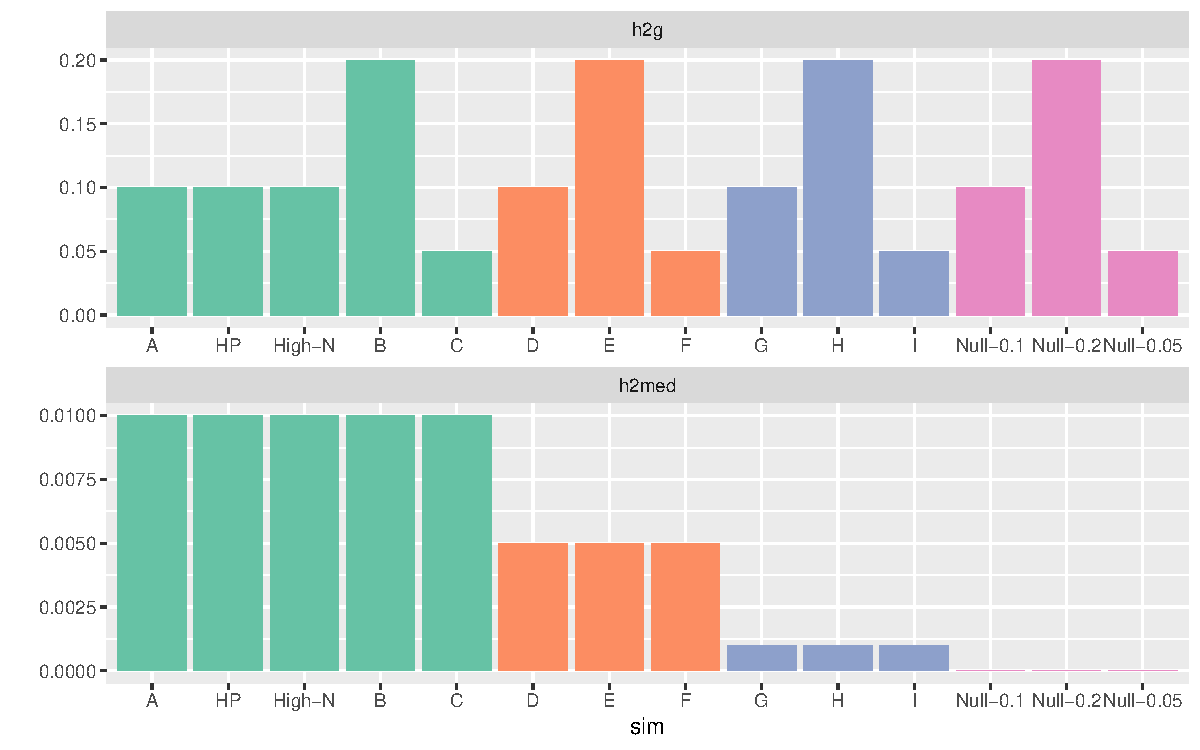
\includegraphics[width=.7\textwidth]{figs/sim_types}
  \caption{Diagram of the 12 types of \texttt{twas\_sim} simulations
    performed, varying eQTL $h^2$ (top row) and trait variance explained
    through gene expression (bottom row), with 20 replicates of each
    setting resulting in 240 simulations total.}
\end{figure}

\begin{figure}[!ht]
  \centering
  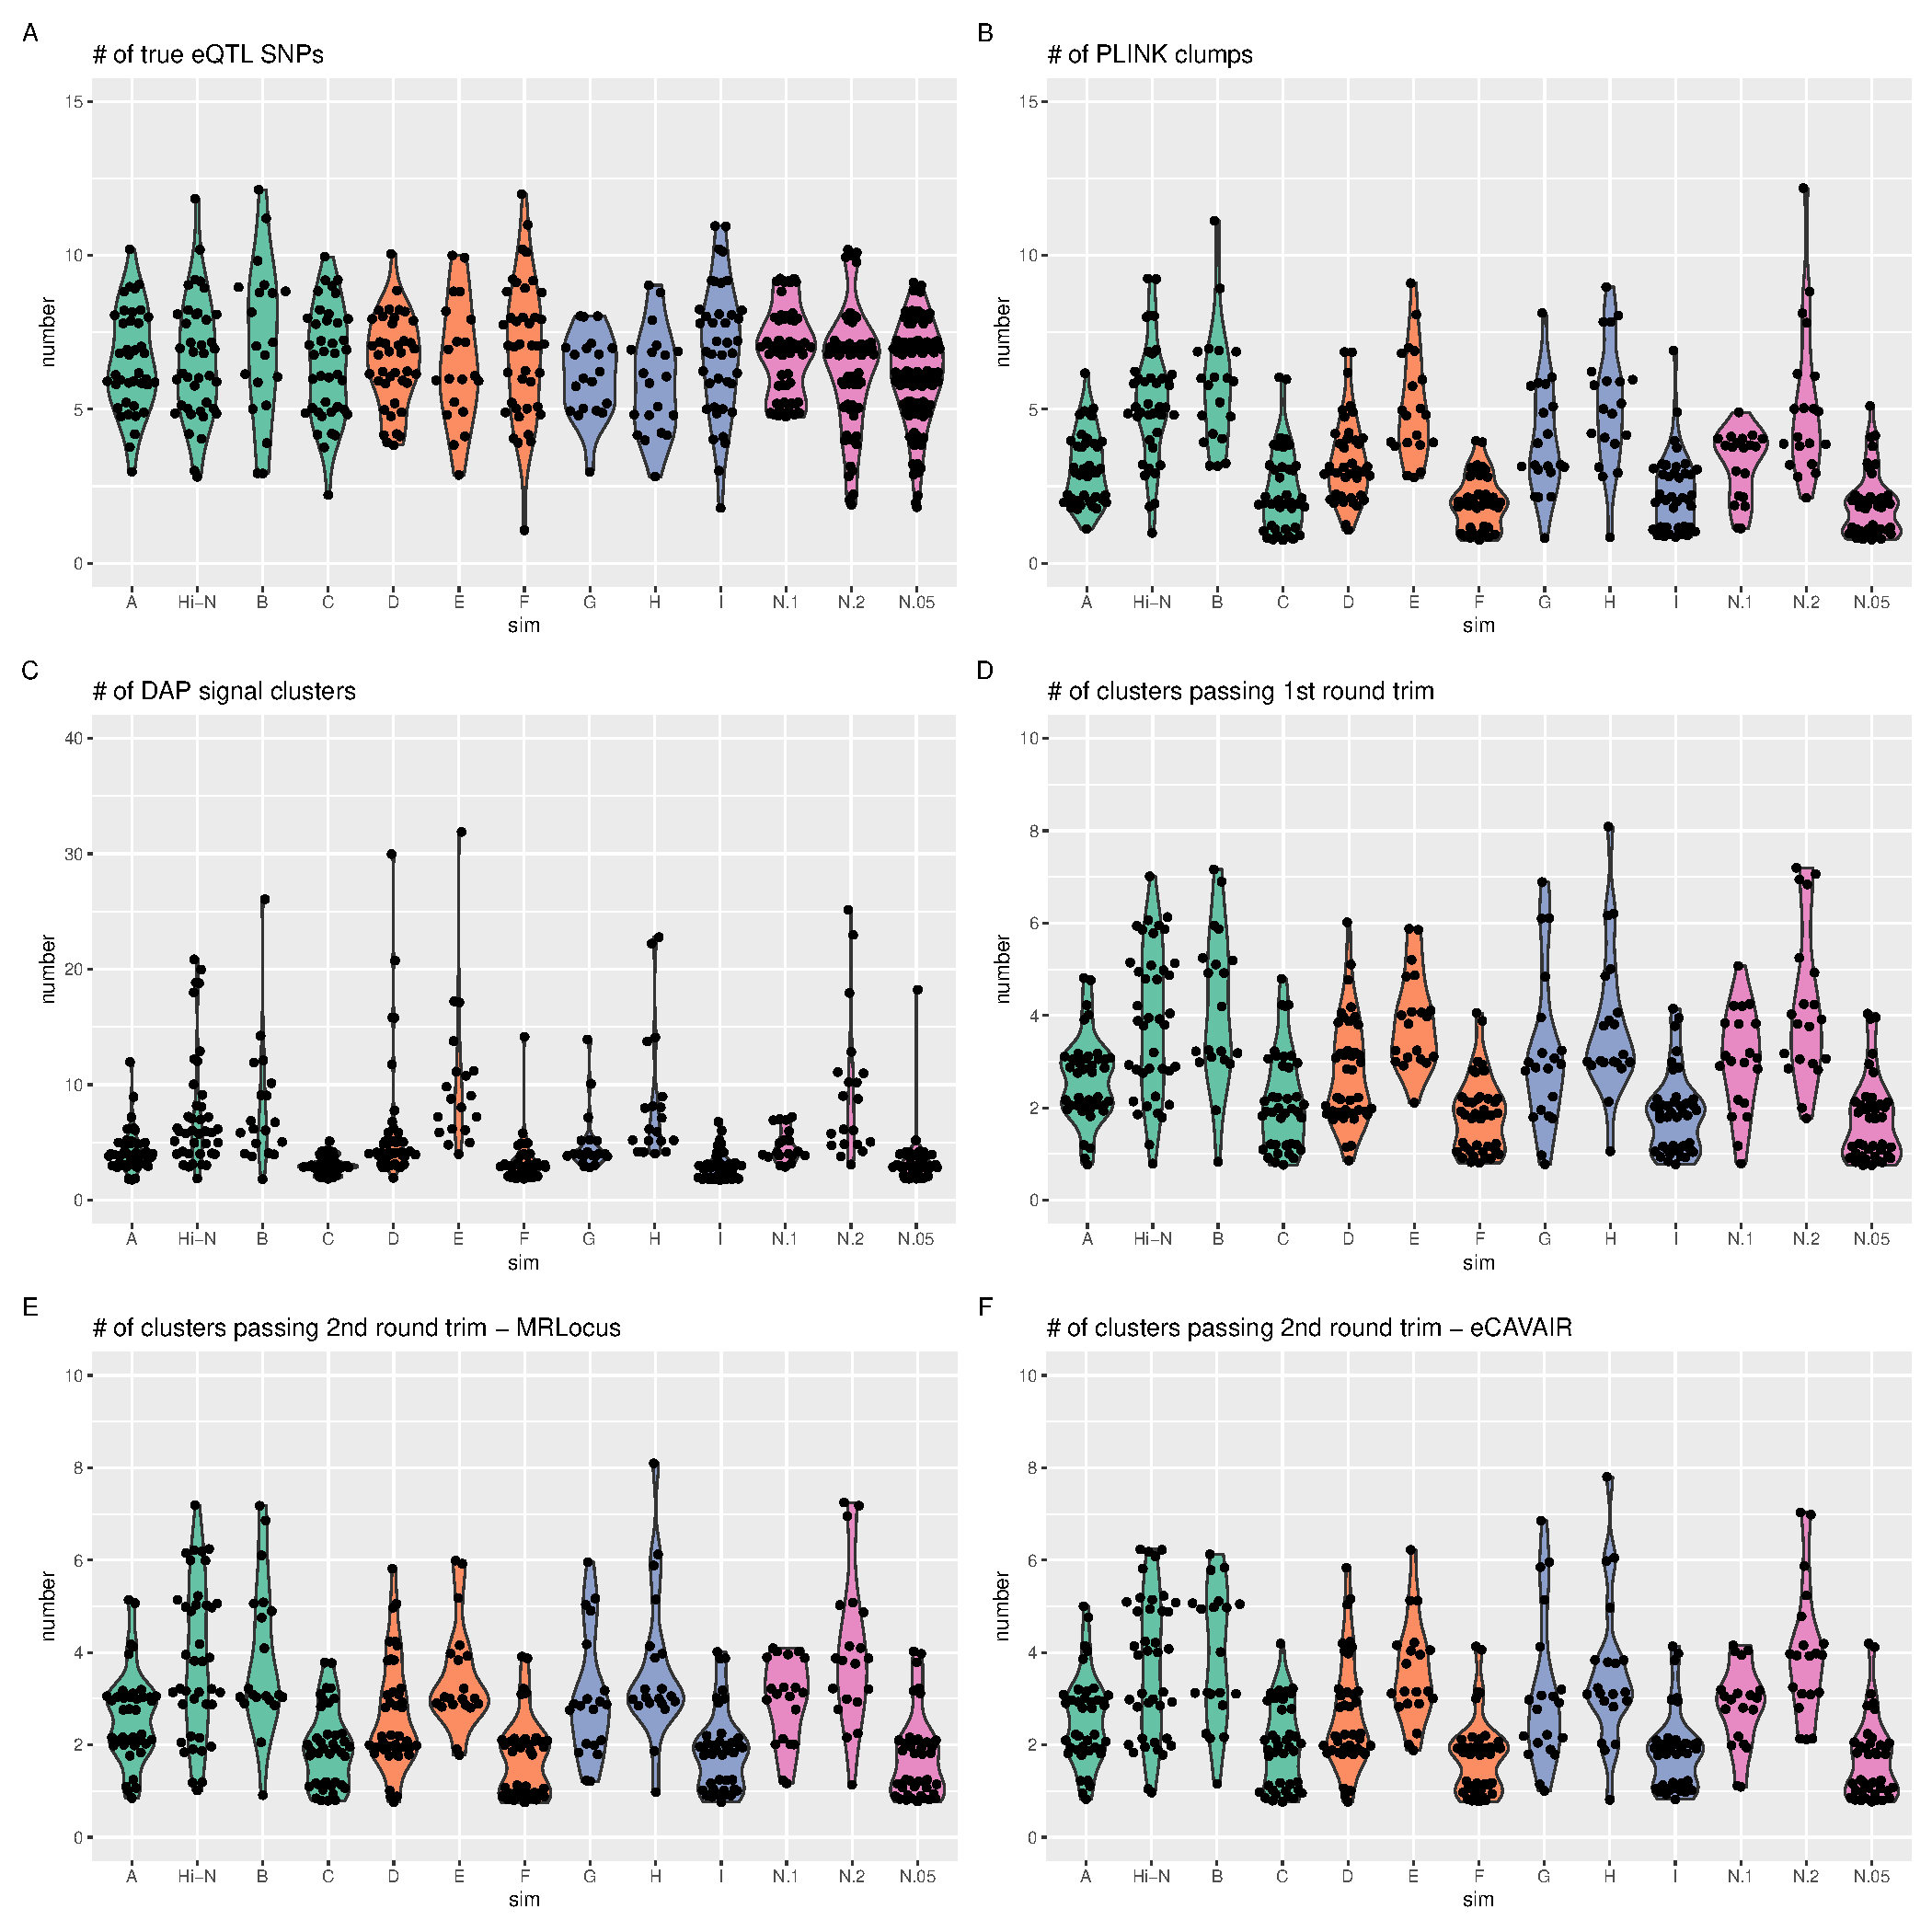
\includegraphics[width=\textwidth]{figs/sim_details}
  \caption{Number of (A) true eQTL SNPs, (B) PLINK clumps, and (C) DAP
    signal clusters per simulation.}
\end{figure}

\begin{figure}[!ht]
  \centering
  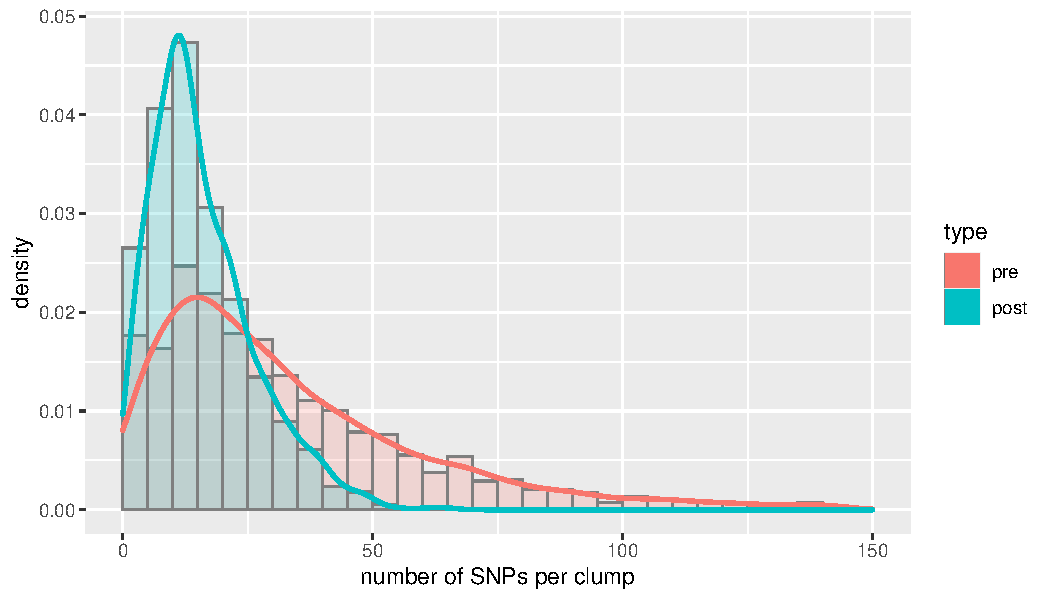
\includegraphics[width=.7\textwidth]{figs/snps-per-clump}
  \caption{SNPs per clump in the 240 simulations, before and after
    collapsing with MRLocus’ collapseHighCorSNPs. The mean number of
    SNPs per clump was 19.9 and 8.8, and the median number of SNPs per
    clump was 15 and 8 (before and after, respectively).} 
\end{figure}

\begin{figure}[!ht]
  \centering
  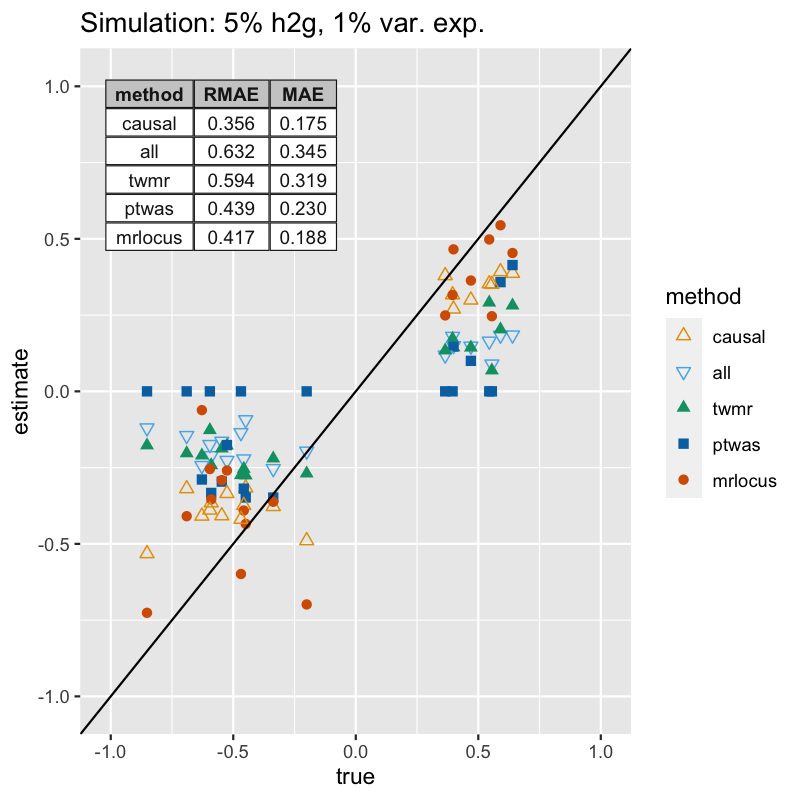
\includegraphics[width=.7\textwidth]{figs/sim2.png}
  \caption{Accuracy of gene-to-trait effect estimation across 8
    additional non-null simulations.} 
\end{figure}

\begin{figure}[!ht]
  \centering
  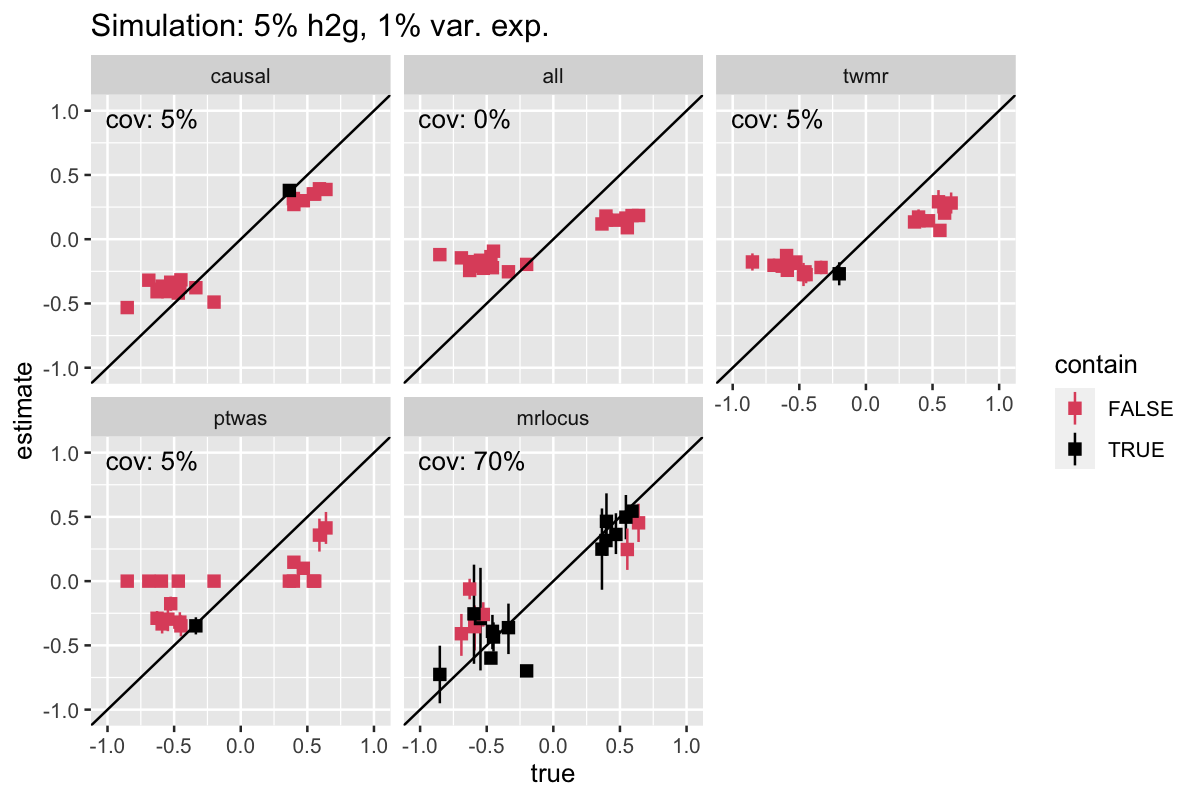
\includegraphics[width=\textwidth]{figs/cover2.png}
  \caption{Coverage of confidence or credible intervals for the
    gene-to-trait effect across 8 additional non-null simulations.}
\end{figure}

\begin{figure}[!ht]
  \centering
  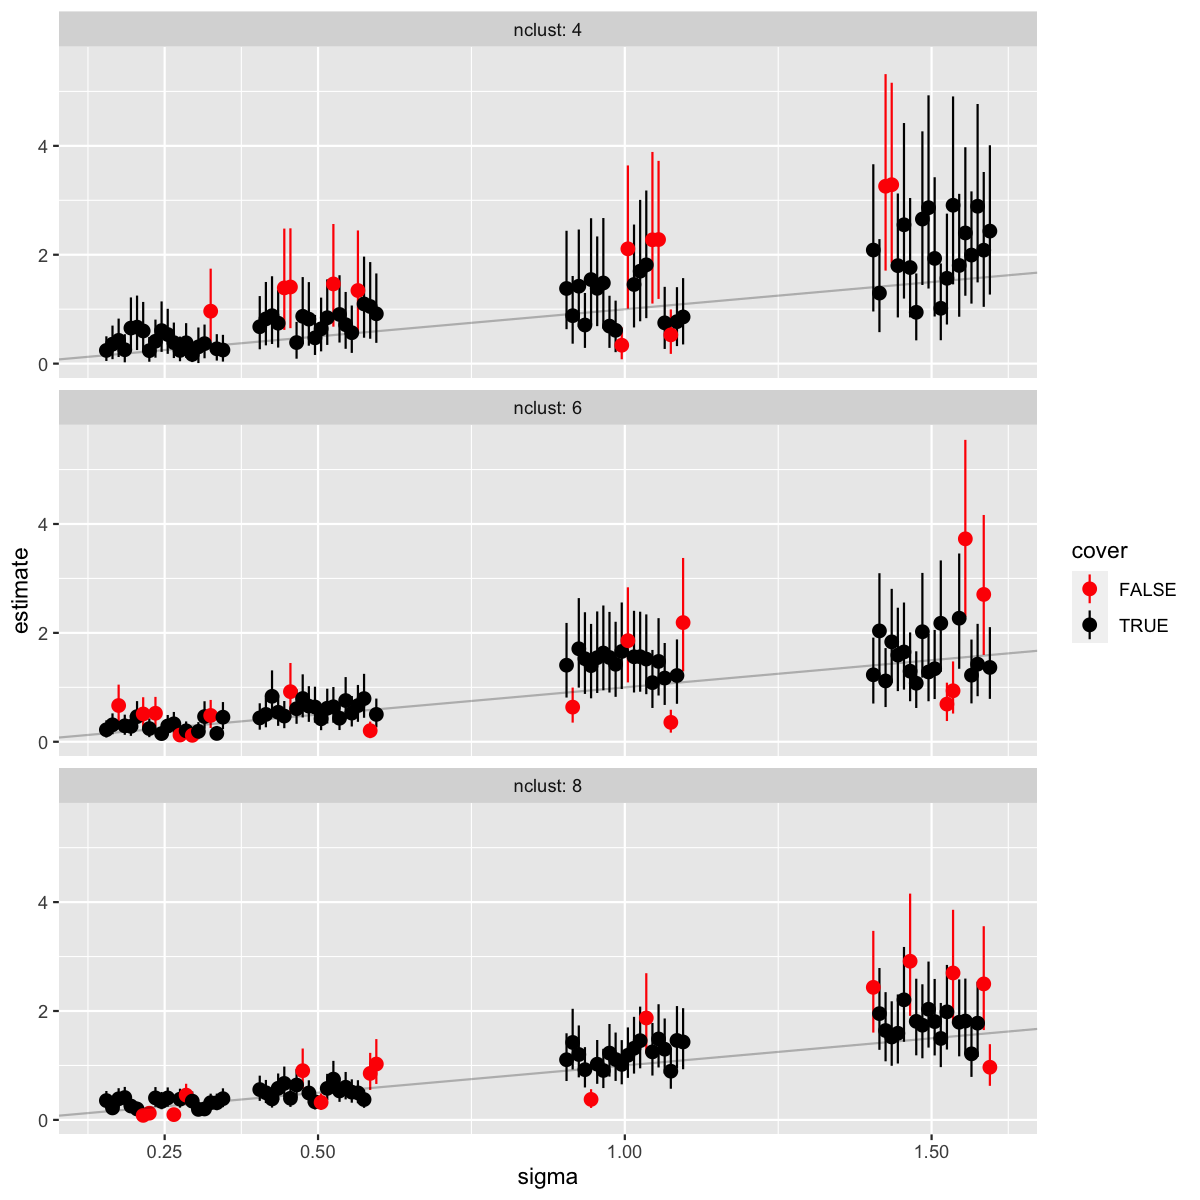
\includegraphics[width=\textwidth]{figs/sigma_est.png}
  \caption{Simulation assessing MRLocus' estimation of the scale of
    dispersion of effects ($\sigma$) around the gene-to-trait fitted
    line. The summary statistics for eQTL and GWAS were generated from
    a multivariate normal distribution as in the eCAVIAR model, using
    a simulated LD matrix. The true alpha was set to 1, the true $\sigma$
    varied from 0.25 to 1 in increments of 0.25 (x-axis), and the
    number of LD-independent clusters varied between 4, 6, and 8
    (left, middle, and right panels), with 10 iterations per setting
    (plotted with spacing to avoid overplotting). The posterior mean
    is indicated with a dot, while 80\% quantile-based credible
    intervals and their coverage of the true value are indicated with
    the line and its color. The simulation script is included within
    the MRLocus package in the test directory, as an R script
    \texttt{"test\_sigma.R"}.} 
\end{figure}

\begin{figure}[!ht]
  \centering
  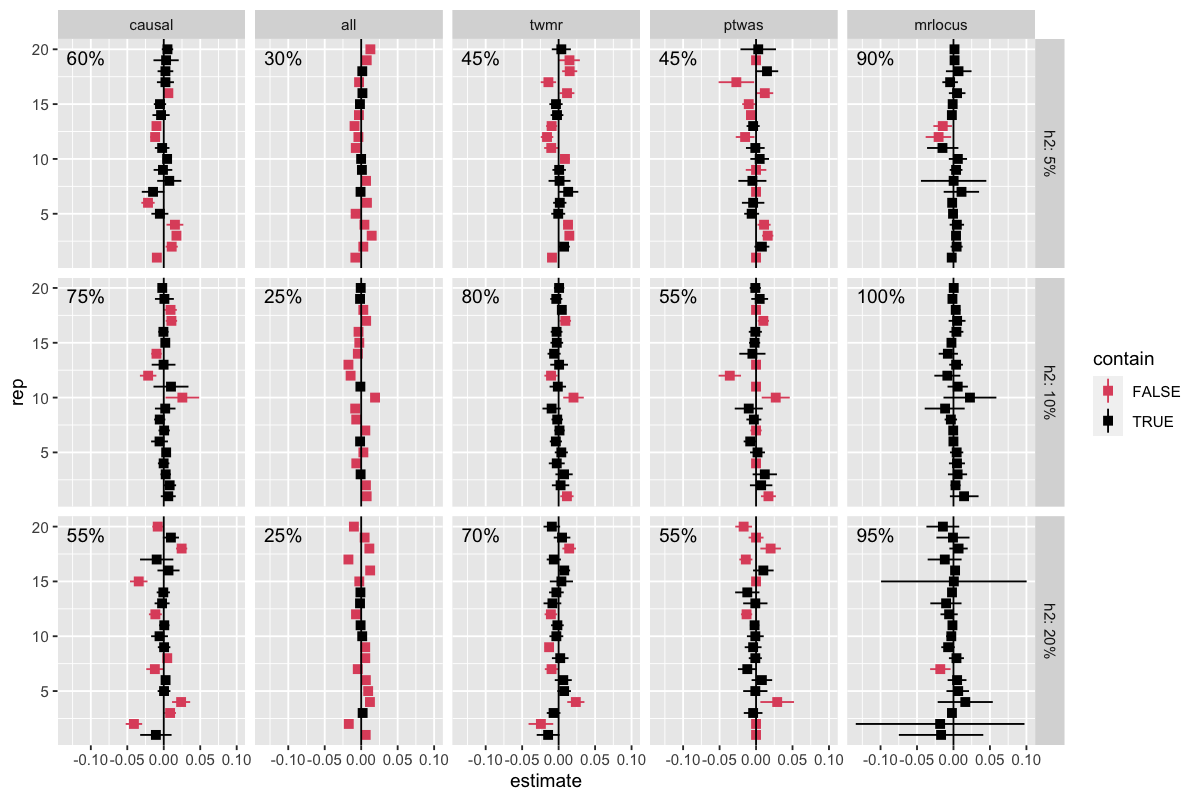
\includegraphics[width=\textwidth]{figs/nullplot.png}
  \caption{Coverage of confidence or credible intervals for the 3 null
    simulation settings.}
\end{figure}

\begin{figure}[!ht]
  \centering
  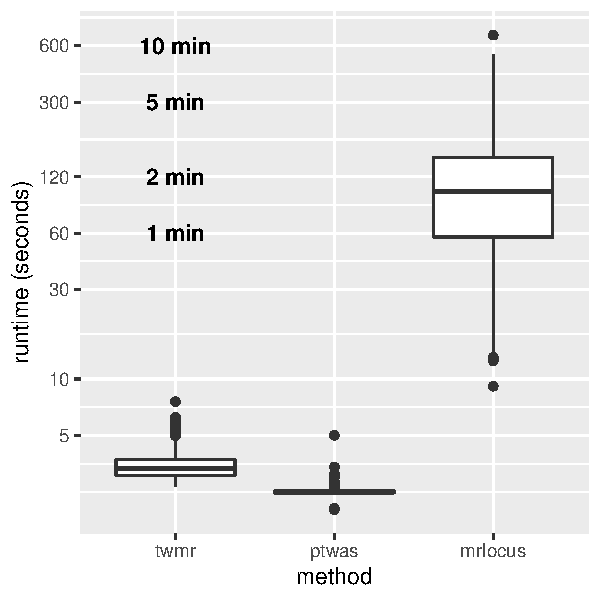
\includegraphics[width=.7\textwidth]{figs/runtime}
  \caption{Runtime for TWMR, PTWAS, and MRLocus on the 240
    simulations. The runtime for a single locus using a single core is
    shown on the y-axis.}
\end{figure}

\end{document}
